The Drupal service at CERN supports website admins to host and administer websites directed to the grand public,
such as experiment or departmental central websites.
Some of the most popular sites based on this service are \href{https://home.cern/}{home.cern}, \href{https://atlas.cern}{atlas.cern},
\href{https://cms.cern}{cms.cern}, \href{https://careers.cern}{careers.cern} and \href{https://visit.cern}{visit.cern}.
As such they form CERN's main outreach channel and are critical for the Organization's reputation.

The responsibility of site building at CERN often falls on administrative personnel, or personnel with little technical background in web technologies.
This in turn shapes the kind of service we provide; contrary to best practices, it is for example impractical to rely exclusively on developer-centric workflows like GitOps and CLI tools.
A small fraction of our user base, however, have indeed web development experience.

The consequence is that the Drupal service has a dual mission:
\begin{enumerate}
\item to ensure the high availability of these communication channels
\item to simplify administration and site building for the wide-ranging user base
\end{enumerate}

This work describes an infrastructure project that focuses on furthering the first mission, without sacrificing the second.
Ideally, the changes should be almost transparent for non-technical site administrators, while enabling previously unavailable best-practices workflows for technical users.


\subsection{Load characteristics}

\begin{figure}[h]
\centering
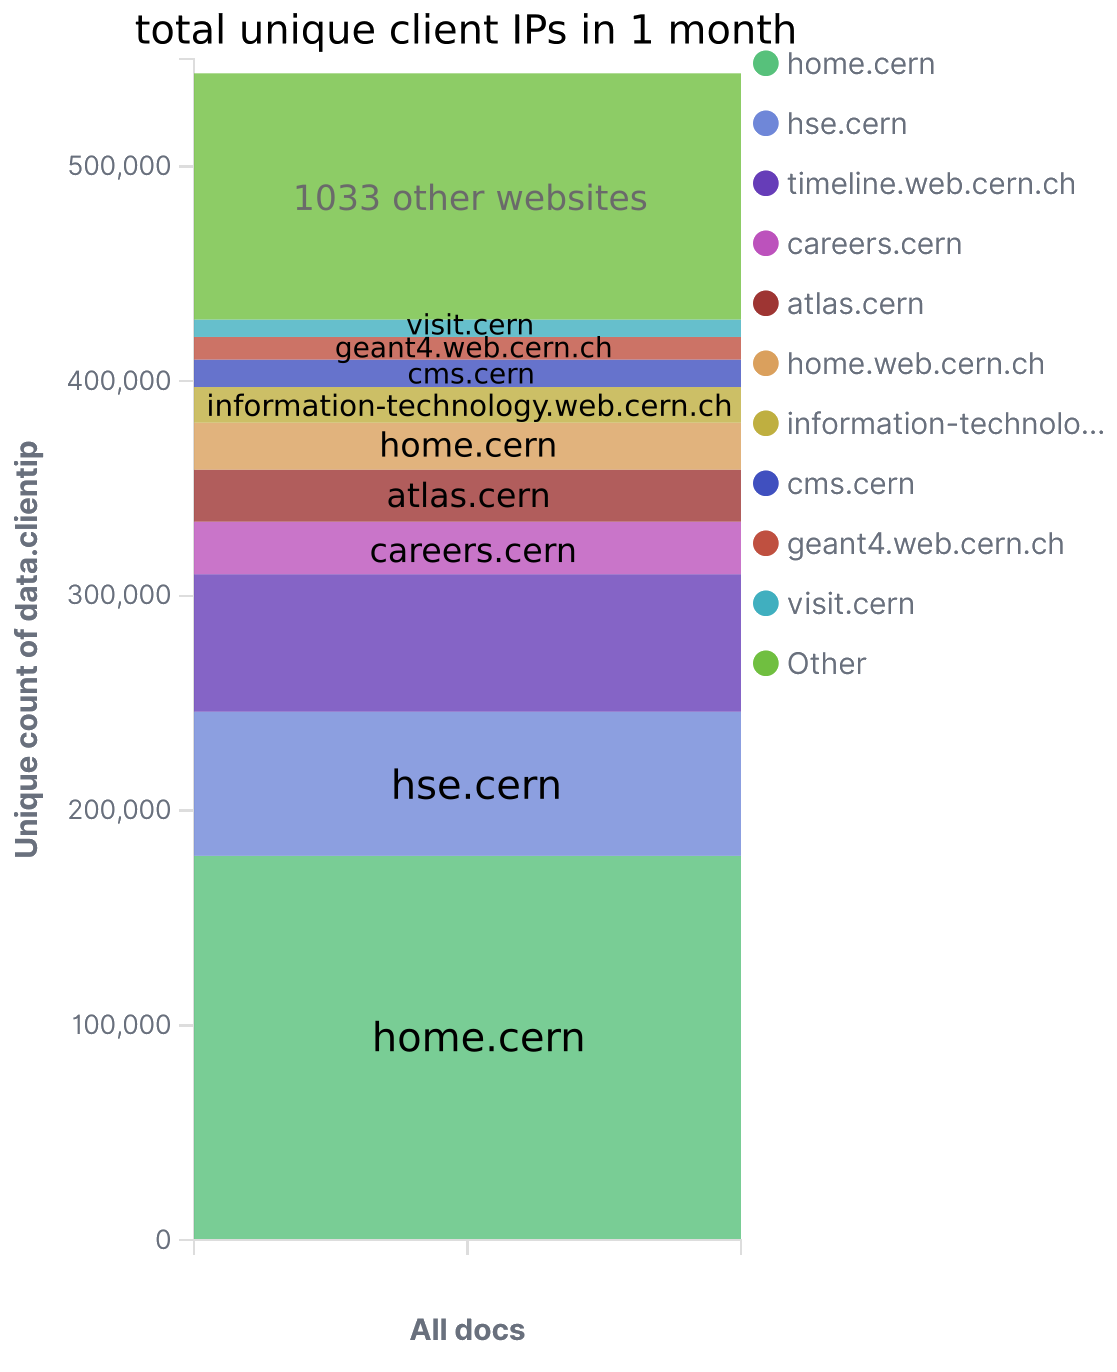
\includegraphics[width=.5\textwidth]{figures/drupal-top10-uniqClientIP.png}
\caption{Calculating the unique client IPs over a month from Apache logs and grouping per site
is taken as a proxy measure of a site's publicity, or how much impact it has on the Organization's reputation.
In this figure the top 10 most public Drupal websites are shown.
home.cern appears twice as home.cern and home.web.cern.ch (but it's the same website)
}
\label{fig-1}       % Give a unique label
\end{figure}
<graph: kibana top10 uniqueIP stacked bar> %  https://monit-timber-drupal-prod8.cern.ch/kibana/app/kibana#/visualize/create?type=histogram&indexPattern=d2ef41c0-e515-11e9-886e-69c303354aa9&_g=(refreshInterval:(pause:!t,value:0),time:(from:now-1M,to:now))&_a=(filters:!(),linked:!f,query:(language:kuery,query:'data.program:%22httpd%22'),uiState:(),vis:(aggs:!((enabled:!t,id:'1',params:(field:data.clientip),schema:metric,type:cardinality),(enabled:!t,id:'2',params:(field:data.sitename,missingBucket:!f,missingBucketLabel:Missing,order:desc,orderBy:'1',otherBucket:!t,otherBucketLabel:Other,size:10),schema:group,type:terms)),params:(addLegend:!t,addTimeMarker:!f,addTooltip:!t,categoryAxes:!((id:CategoryAxis-1,labels:(show:!t,truncate:100),position:bottom,scale:(type:linear),show:!t,style:(),title:(),type:category)),grid:(categoryLines:!f),legendPosition:right,seriesParams:!((data:(id:'1',label:'Unique%20count%20of%20data.clientip'),drawLinesBetweenPoints:!t,mode:stacked,show:true,showCircles:!t,type:histogram,valueAxis:ValueAxis-1)),times:!(),type:histogram,valueAxes:!((id:ValueAxis-1,labels:(filter:!f,rotate:0,show:!t,truncate:100),name:LeftAxis-1,position:left,scale:(mode:percentage,type:linear),show:!t,style:(),title:(text:'Unique%20count%20of%20data.clientip'),type:value))),title:'New%20Visualization',type:histogram))

<graph: kibana top10 requests stacked bar> %  https://monit-timber-drupal-prod8.cern.ch/kibana/app/kibana#/visualize/create?type=histogram&indexPattern=d2ef41c0-e515-11e9-886e-69c303354aa9&_g=(filters:!(),refreshInterval:(pause:!t,value:0),time:(from:now-1M,to:now))&_a=(filters:!(('$state':(store:appState),meta:(alias:!n,disabled:!f,index:d2ef41c0-e515-11e9-886e-69c303354aa9,key:data.sitename,negate:!t,params:(query:test-jardin-de-particules-d8.web.cern.ch),type:phrase,value:test-jardin-de-particules-d8.web.cern.ch),query:(match:(data.sitename:(query:test-jardin-de-particules-d8.web.cern.ch,type:phrase)))),('$state':(store:appState),meta:(alias:!n,disabled:!f,index:d2ef41c0-e515-11e9-886e-69c303354aa9,key:data.sitename,negate:!t,params:(query:test-uo-bat.web.cern.ch),type:phrase,value:test-uo-bat.web.cern.ch),query:(match:(data.sitename:(query:test-uo-bat.web.cern.ch,type:phrase)))),('$state':(store:appState),meta:(alias:!n,disabled:!f,index:d2ef41c0-e515-11e9-886e-69c303354aa9,key:data.sitename,negate:!t,params:(query:test-lpcc.web.cern.ch),type:phrase,value:test-lpcc.web.cern.ch),query:(match:(data.sitename:(query:test-lpcc.web.cern.ch,type:phrase)))),('$state':(store:appState),meta:(alias:!n,disabled:!f,index:d2ef41c0-e515-11e9-886e-69c303354aa9,key:data.sitename,negate:!t,params:(query:test-missionlhc.web.cern.ch),type:phrase,value:test-missionlhc.web.cern.ch),query:(match:(data.sitename:(query:test-missionlhc.web.cern.ch,type:phrase))))),linked:!f,query:(language:kuery,query:'data.program:%22httpd%22'),uiState:(),vis:(aggs:!((enabled:!t,id:'1',params:(),schema:metric,type:count),(enabled:!t,id:'2',params:(field:data.sitename,missingBucket:!f,missingBucketLabel:Missing,order:desc,orderBy:'1',otherBucket:!t,otherBucketLabel:Other,size:10),schema:group,type:terms)),params:(addLegend:!t,addTimeMarker:!f,addTooltip:!t,categoryAxes:!((id:CategoryAxis-1,labels:(show:!t,truncate:100),position:bottom,scale:(type:linear),show:!t,style:(),title:(),type:category)),grid:(categoryLines:!f),legendPosition:right,seriesParams:!((data:(id:'1',label:Count),drawLinesBetweenPoints:!t,mode:stacked,show:true,showCircles:!t,type:histogram,valueAxis:ValueAxis-1)),times:!(),type:histogram,valueAxes:!((id:ValueAxis-1,labels:(filter:!f,rotate:0,show:!t,truncate:100),name:LeftAxis-1,position:left,scale:(mode:percentage,type:linear),show:!t,style:(),title:(text:Count),type:value))),title:'New%20Visualization',type:histogram))


\href{https://home.cern/}{home.cern} is the most public website at CERN.
Out of 1043 Drupal websites currently hosted, it alone serves 32\% of monthly unique visitors.
The top 10 websites together serve 79\% of all unique visitors, leaving only 1/5 among them headed for the other 1033 websites.
This is an intrinsic characteristic of the service load, which is heavily skewed towards a very small number of critical websites.

Unique visitors is a good measure of a website's publicity, but a measure that is easier to assess an infrastructure on is the number of HTTP requests.
The situation there is similar, with the top 10 websites being the target of 60\% of all requests.
In section \ref{sec-experiment} we will describe an experiment on resource optimization by assigning websites to different Quality of Service classes,
according to their needs, where both metrics are relevant.


\subsubsection{Concurrent requests}

< graph KIBANA simultaneous requests across infra> %  https://monit-timber-drupal-prod8.cern.ch/kibana/app/kibana#/visualize/create?type=histogram&indexPattern=d2ef41c0-e515-11e9-886e-69c303354aa9&_g=(refreshInterval:(pause:!t,value:0),time:(from:now-2500s,to:now-2250s))&_a=(filters:!(),linked:!f,query:(language:kuery,query:'data.program:%22httpd%22'),uiState:(),vis:(aggs:!((enabled:!t,id:'1',params:(),schema:metric,type:count),(enabled:!t,id:'2',params:(customInterval:'2h',drop_partials:!f,extended_bounds:(),field:metadata.timestamp,interval:s,min_doc_count:1,timeRange:(from:now-1h,to:now),useNormalizedEsInterval:!t),schema:segment,type:date_histogram)),params:(addLegend:!t,addTimeMarker:!f,addTooltip:!t,categoryAxes:!((id:CategoryAxis-1,labels:(show:!t,truncate:100),position:bottom,scale:(type:linear),show:!t,style:(),title:(),type:category)),grid:(categoryLines:!f),legendPosition:right,seriesParams:!((data:(id:'1',label:Count),drawLinesBetweenPoints:!t,mode:stacked,show:true,showCircles:!t,type:histogram,valueAxis:ValueAxis-1)),times:!(),type:histogram,valueAxes:!((id:ValueAxis-1,labels:(filter:!f,rotate:0,show:!t,truncate:100),name:LeftAxis-1,position:left,scale:(mode:normal,type:linear),show:!t,style:(),title:(text:Count),type:value))),title:'New%20Visualization',type:histogram))

The entire infrastructure in regular situations handles peaks of up to 250 concurrent requests per second.


% NOTES
Tell a story about who visits the Drupal infra.
Show Kibana graphs:
- as a whole
- for top 10 websites
- for home.cern
- per minute (simultaneous)
=> define num of users for QoS classes
% NOTES

\subsection{Users of the infrastructure}

Although the load to the infrastructure comprises website visitors, the users that define the functional requirements of this system are website administrators: site builders and web developers.

Technical and non-technical users.
Pick smt from White Area talk.

\subsection{Existing infrastructure}
\label{old-infra}

- physical linux servers with NAS
- haproxy -> nginx -> php-fpm
- static physical size
- poor site isolation: multisite drupal with linux users